\subsection{Programmierschnittstellen}
\label{subsec:Programmierschnittstellen}

Auf der Leiterplatte des PartyMixers sind der Mikrocontroller und das WiFi-Modul (Targets), welche programmiert werden müssen. Damit die Software vom Computer (Host) auf die Komponenten geladen werden kann, braucht es eine Programmierschnittstelle. Computerseitig geschieht dies über USB.
Die Übermittlung von Daten über die USB-Schnittstelle geschieht über ein differentielles Verfahren und benötigt zwei Kommunikationsleitungen (D+ und D-), welche innerhalb des USB-Kabels verdrillt sind. Das differentielle Verfahren zeichnet sich dadurch aus, dass elektromagnetische Störungen von ausserhalb zu einem grossen Teil eliminiert werden können, da sie sich auf beide Leitungen gleich auswirken. Die Targets werden jedoch über eine serielle Schnittstelle programmiert und benötigen zusätzliche Steuerleitungen um in einen Programmiermodus zu kommen. Deswegen wird ein USB-UART-Konverter verwendet, der das USB-Signal in ein UART-Signal wandelt und die entsprechenden Steuerleitungen zur Verfügung stellt. 

Die beiden Programmierschnittstellen benötigen unterschiedlich viele Steuerleitungen, da sie sich im Verfahren zum Aufruf des Download-Boot-Modus unterscheiden. Die Verfahren sind vom Hersteller des Targets gegeben und können nicht beeinflusst werden.
%Im Anhang Kapitel \ref{Appendix:Handshake_uC} und \ref{Appendix:Handshake_ESP} wird dargestellt, welche Leitungen für das jeweilige Flash-Interface benötigt werden.
Die vom Verfahren vorgegebene Signalfolge, welche an den vordefinierten Pins angelegt werden muss, um den Programmier-Modus zu starten, wird auch Handshake genannt. Dieser findet immer statt, bevor ein Programm vom Host auf ein Target geladen wird.
Er wird vom Host gesteuert und muss deswegen im Voraus bekannt sein, sodass die gewünschte Signalfolge berücksichtigt werden kann.
%Dieser wird in den Kapiteln \ref{subsubsec:Handshake_ATMega2560} und \ref{subsubsec:Handshake_ESP32} beschrieben. In Kapitel \ref{subsubsec:USB-B} wird dann das Schema beschrieben.
%Die USB-B-seitige Schnittstelle wird an den Computer angeschlossen und muss nicht häher betrachtet werden.

\paragraph{Handshake Mikrocontroller}\mbox{}

Um Download-Boot-Modus des Mikrocontrollers zu starten, reicht es, die Reset-Leitung per Handshake auf 0V zu ziehen. Dies wird erreicht, indem das Wiring-Protokoll verwendet wird, das auf den verwendeten Bootloader auf dem Mikrocontroller angepasst ist und bei Ausführen des Handshakes die DTR- bzw. Reset-Leitung toggelt. Nachdem der Handshake ausgeführt wurde und das Programmiertool AVRdude die Device-Signatur des Mikrocontrollers (0x1E9801) verifiziert hat, sendet es das kompilierte HEX-File an den Mikrocontroller.

%Um die Daten hochladen zu können, muss sichergestellt werden, dass avrdude mit dem stk500v2 programmer hochlädt und die DTR-Leitung toggelt, bevor der Programmiervorgang stattfindet. Die DTR-Leitung hängt über einen Kondensator an der Reset-Leitung und zieht diese auf GND, womit der Bootloader des ATMega2560 aktiv wird. Deswegen wird beim Hochladen in AVRdude als programming-id der \textit{wiring}-programmer angegeben, sichtbar in Kapitel \ref{Appendix:AVR_STK500} (-c wiring).

\paragraph{Handshake WiFi-Modul}\mbox{}

Um Download-Boot-Modus des WiFi-Moduls zu starten, sind die Strapping Pîns relevant. Sie werden nach einem Neustart des WiFi-Moduls als Erstes gelesen und bestimmen den Grundzustand des WiFi-Moduls. Die Tabelle \ref{tab:Einfluss_Pins_auf_Boot_Modus} zeigt die Strapping-Pins und deren Einfluss auf den Boot-Modus. Aufgrund der defaultmässigen Pull-up und -down Widerstände kann aus dieser interpretiert werden, dass wenn U0TXD, IO2 und IO5 ''floating'' sind, IO0 den Boot-Modus bestimmt \cite[S.12-S.14]{espressif_systems_esp32_2016}. Mittels Handshake wird die Resetleitung getoggelt und die Strapping-Pins so gesetzt, dass der Download-Boot-Modus gestartet wird.

%Im Anhang Kapitel \ref{Appendix:ESP32_Strapping} sind die erwähnten Strapping-Pins aufgelistet. Mit diesen Pins kann nebst dem Bootmodus die Ausgangsspannung des internen Spannungsregler für VDD\_SDIO, der Debug-Log-Print während dem Booten sowie das SPI-Timing der Kommunikation mit der SDIO-Schnittstelle des WiFi-Moduls konfiguriert werden. Eine genauere Beschreibung der Pins befindet sich im selben Kapitel.

\begin{table}[H]
\center
\begin{tabular}{|l|c|c|c|}
\hline
\multicolumn{4}{|c|}{\textbf{Boot-Mode Konfiguration}}\\
\hline
\textbf{Pin} & \textbf{Default} & \textbf{Boot} & \textbf{Download} \\
\hline
IO0 & 1 & 1 & 0 \\
\hline
U0TXD & 1 & 1 & Don't care \\
\hline
IO2 & 0 & Don't care & 0 \\
\hline
IO15 & 1 & Don't care & Don't care \\
\hline
IO5 & 1 & 1 & Don't care \\
\hline
\end{tabular}
\caption{Wenn U0TXD, IO2, IO5 floating sind, bestimmt IO0 den Boot-Modus.}
\label{tab:Einfluss_Pins_auf_Boot_Modus}
\end{table}

Im Folgenden wird die Hardware für die Programmierschnittstellen beschrieben. Es ist darauf zu achten, dass in Abbildung \ref{fig:Schema_USB_B} nur das Schema für die Programmierschnittstelle des WiFi-Moduls zu sehen ist. Vorab: Bei den Leitungen DTR, DSR, RTC, CTS, RXD und TXD handelt es sich um die Kommunikationsleitungen zwischen dem USB-UART-Konverter und dem Target. In Tabelle \ref{tab:USB_ESP} sind die Unterschiede tabellarisch aufgelistet.

\begin{table}[H]
\center
\begin{tabular}{|c|lcl|c||l|}
\hline
\textbf{Leitung} & & & & \textbf{Konverter} & \textbf{Target} \\ \hline
RXD & <== & über Widerstand & === & TX & beide \\
TXD & === & über WIderstand & ==> & RX & beide\\
IO\_0 / Reset & <== & über Transistor & === & DTR & beide\\
EN & <== & über Transistor & === & RTS & nur WiFi-Modul\\
IO\_13 & <== & über Widerstand & === & RTS & nur WiFi-Modul\\
IO\_15 & <== & über Widerstand & === & CTS & nur WiFi-Modul\\
\hline
\end{tabular}
\caption{Verbindung zwischen USB und WiFi-Modul.}
\label{tab:USB_ESP}
\end{table}

\paragraph{Schema}\mbox{}

Das USB-Kabel wird an der Buchse J2 angeschlossen. Sobald ein USB-Kabel eingesteckt ist, sind die Leiterplatine und der Computer auf gleichem Ground-Potential und die Leitungen D+ und D- mit dem Konverter verbunden. Über das USB-Kabel werden ebenfalls 5V am Spannungsteiler R12 und R13 angelegt, was vom Konverter als bestehende USB-Verbindung interpretiert wird. Da beim Einstecken die Gefahr von Spannungsdifferenzen besteht, wird ein ESD-Schutz benötigt, welcher vom den Dioden D2-4 gewährleistet wird. Die LED's können verwendet werden, um einen Datenfluss zu signalisieren. Die Widerstände in den Kommunikations- und Steuerleitungen schützen die Pins vor Ausgleichsströmen, die entstehen wenn die Pins auf unterschiedlichem Potential liegen.
\begin{figure}[h!]
	\centering
	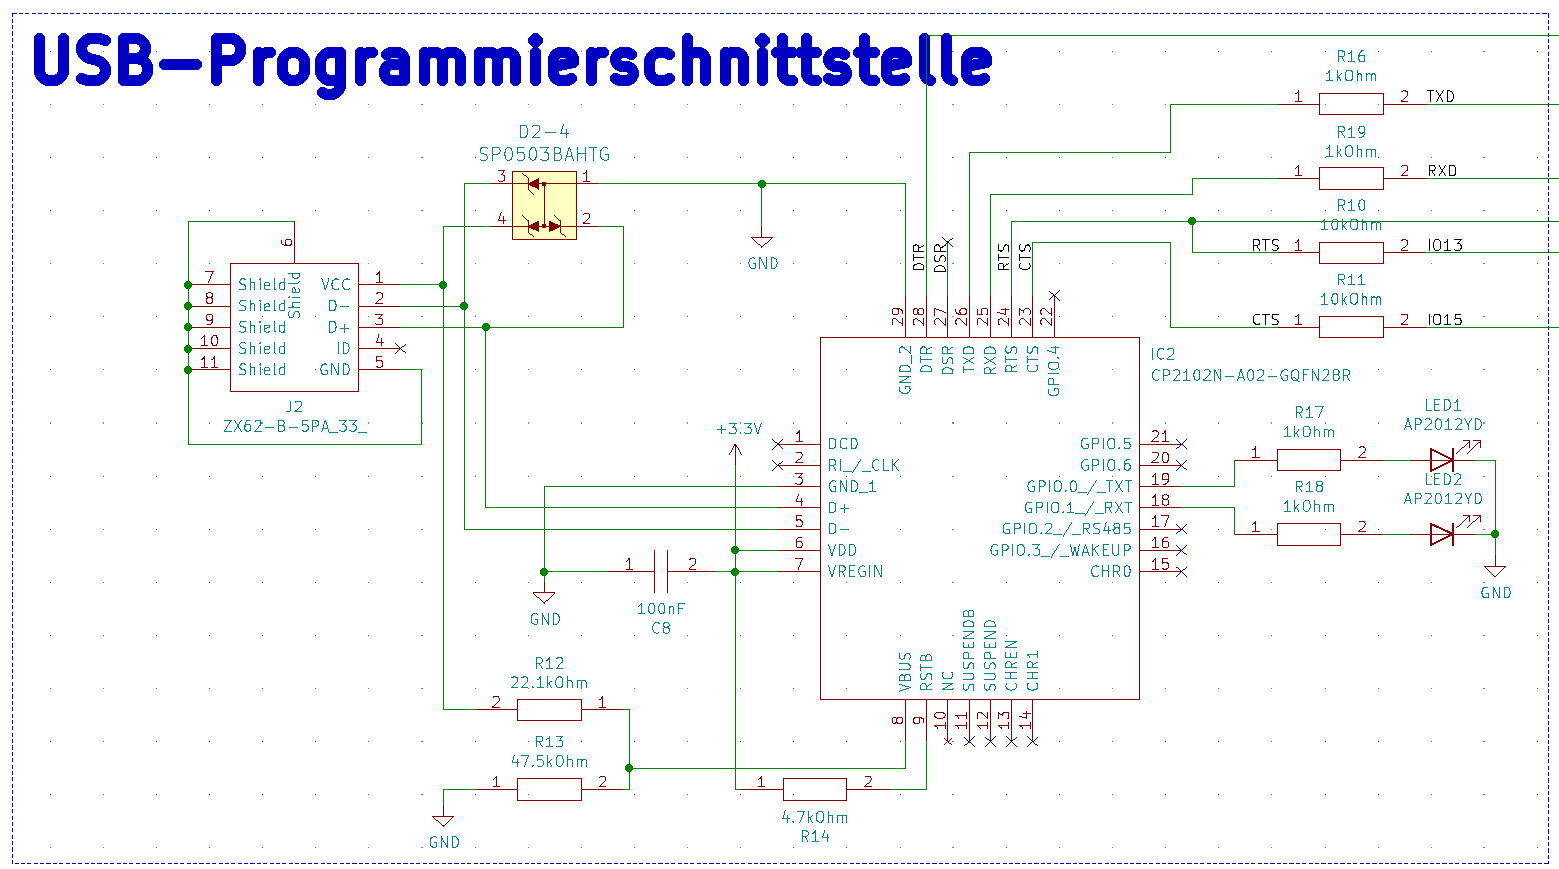
\includegraphics[width=1\textwidth]{graphics/Schema_USB_B}
	\caption{Schema USB-B.}
	\label{fig:Schema_USB_B}
\end{figure}
\newpage
\paragraph{Funktionsbeschrieb der Schaltung}\mbox{}

Der dazugehörige ESD-Schutz bildet die Diodenschaltung D2-D4. Dabei handelt es sich um ESD-Schutzdioden des Typs SP0503BAHTG. Sie werden ab einer Spannung von 3.3V leitend und reduzieren so die maximale Spannung auf den Eingangspins des Konverters auf 3.3V. Der Konverter hat im Schema die Bezeichnung IC2. Es ist ein CP2102N des Herstellers Silicon-Labs. Die Widerstände R12 und R13 bilden einen Spannungsteiler, welcher an die 5V-Eingangsspannung der Buchse angeschlossen ist. Der Spannungsteiler hat eine 3.3V Zwischenspannung und ist an dem VBUS-Eingang des Konverters angeschlossen. Die Widerstände R16, R19, R10 und R11, welche die Ausgleichsströme zwischen dem USB-UART-Konverter und den Targets begrenzen, sind mit 1k\textOmega dimensioniert. Der Widerstand R14 ist ein Pull-Up Widerstand, welcher den Konverter permanent aktiviert und ist mit 4.7k\textOmega dimensioniert. Die Widerstände R17 und R18 reduzieren den Strom durch die LEDs vom Typ AP2012YD.